% Section: cross_platform (\input from main.tex)
\section{Cross-Platform Comparison}
\label{sec:cross}

The three platforms differ in core count (10, 4 and 2), in core types (A mixes
performance and efficiency cores), in instruction set and memory model (ARMv8
on A and B, x86-64 on C), and in operating system and C++ library (macOS with
libc++ on A, Linux with libstdc++ on B and C). Platforms A and B run on the
same Apple M5 chip, natively and inside a virtual machine.
Table~\ref{tab:cross} summarizes the best result of each part on each platform,
and Figure~\ref{fig:cross} compares how the key results scale.

\begin{table}[H]
\centering
\small
\caption{Best result per platform. ``$\times$'' values are speed-ups over
sequential A* on the same platform; thread counts in parentheses.}
\label{tab:cross}
\begin{tabularx}{\linewidth}{l YYY}
\toprule
 & \textbf{A: macOS, M5, 10 cores} & \textbf{B: Linux VM, 4 vCPU} & \textbf{C: Linux, Xeon, 2 vCPU} \\
\midrule
Sequential A*, Euclidean $h$ (city graph) & 2.2\,ms / query & 2.7\,ms / query & 6.4\,ms / query \\
Best list, 90\% \texttt{contains} & lazy, \texttt{std::mutex}: 15.9\,Mops/s (16) & lazy, TTAS: 8.4\,Mops/s (8) & lazy, TTAS: 3.6\,Mops/s (2) \\
Best list, \texttt{add}/\texttt{removeMin}, $\ge 2$ threads & coarse, backoff: 39.1\,Mops/s (2) & coarse, backoff: 33.5\,Mops/s (2) & coarse, backoff: 19.7\,Mops/s (2) \\
Best parallel A*, Euclidean $h$ & $0.42\times$ (shared heap, 2) & $0.53\times$ (shared heap, 2) & $0.58\times$ (shared heap, \texttt{std::mutex}, 4) \\
Best parallel A*, costly $h$ & $1.35\times$ (\HDA, 4) & $1.44\times$ (\HDA, 4) & $1.67\times$ (shared heap, 4) \\
Best list-based parallel A*, costly $h$ & $1.11\times$ (lazy, 4) & $0.89\times$ (lazy, 8) & $0.74\times$ (lazy, 4) \\
\bottomrule
\end{tabularx}
\end{table}

\begin{figure}[H]
\centering
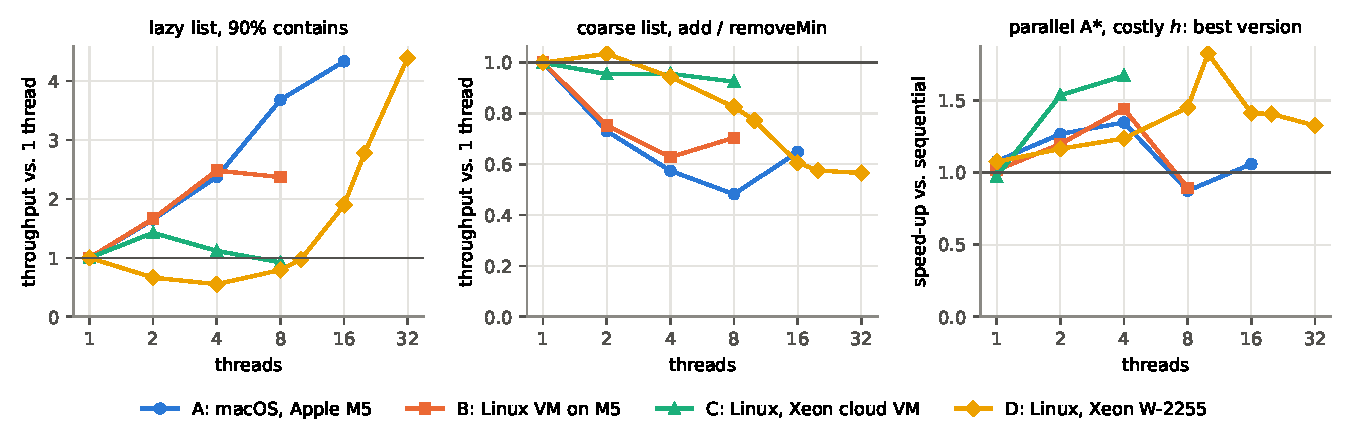
\includegraphics[width=\linewidth]{figures/fig8_cross.pdf}
\caption{Cross-platform scaling: lazy list with the read mix (left), coarse
list with \texttt{add}/\texttt{removeMin} (middle), and the best parallel A*
version at each thread count with the costly heuristic (right).}
\label{fig:cross}
\end{figure}

\textbf{Core count decides how far the lazy list scales.} The lazy list is the
best concurrent set on every platform, and its read throughput keeps growing
for as long as there are cores: up to 16 threads on A ($4.3\times$ with backoff, $5\times$ with \texttt{std::mutex}), 4 on B
($2.5\times$) and 2 on C ($1.4\times$). Its traversals never write shared
memory, so readers do not slow each other down. After the last core, the
curves flatten (A) or fall (B, C).

\textbf{A priority queue at the head does not scale anywhere.}
\texttt{add}/\texttt{removeMin} loses throughput as soon as a second thread
arrives, on every platform and for every list (Figure~\ref{fig:cross},
middle). Many cores do not help when every operation needs the same two
nodes. This is the main reason why parallel A* over a shared OPEN list is
slower than sequential A* on all three machines unless expansions are costly.

\textbf{The granularity of the work matters more than the platform.} With a
cheap heuristic, the best parallel A* is slower than sequential A* on every
platform, and a 10-core laptop does no better than a 2-vCPU cloud machine.
Only with the costly heuristic does parallel A* win on all three platforms
(1.35--1.67$\times$). The best version differs per platform: \HDA, which has no
shared queue, wins on the two ARM platforms; the shared heap wins on the x86 VM.

\textbf{A larger graph helps the lists.} On the city graph OPEN is long, and
several threads can walk it at the same time. The lazy list therefore gains
from extra threads on every platform with the costly heuristic, and on
Platform~A it becomes the first list-based parallel A* that beats sequential
A* ($1.11\times$ at 4 threads). It still loses clearly to the heap at one
thread, because its operations are linear in the size of OPEN.

\textbf{Heterogeneous cores limit Platform~A.} Platform~A has the most cores but
gives the smallest best speed-up for parallel A* (1.35$\times$), and the Linux
VM on the same chip does better with the same 4 threads (1.44$\times$). A search
that all threads share advances at the pace of its slowest thread. From 5
threads on, some threads must run on efficiency cores; macOS may also place
some of the first 4 threads there, whereas the VM's 4 virtual CPUs are
scheduled by the hypervisor. Throughput-oriented code such as the lazy list,
where threads do not wait for each other, uses all 10 cores well.

\textbf{Oversubscription hurts spinning most.} On Platform~C, 4 threads run on 2
virtual CPUs and 8 threads in Part~2. Pure TTAS spinlocks collapse there, and so
does plain \HDA{} ($8\times$ search overhead at 4 threads). Locks and loops that
back off and yield, and the $f$-window for \HDA, keep the damage small. One
result on C we cannot fully explain: the shared heap with the costly heuristic
is fastest at 4 threads on 2 vCPUs ($1.67\times$, against $1.54\times$ at 2
threads), on the city graph as on the small graph. A possible reason is that
the hypervisor gives the VM more physical capacity than 2 vCPUs suggest; we did
not verify this.

\textbf{Memory model.} The same code passed every correctness test on the weak
ARMv8 memory model (A, B) and on x86-64 TSO (C), and ThreadSanitizer found no
data race. Because every shared access uses \texttt{std::atomic} with explicit
acquire/release ordering, no platform-specific code was needed.
